\chapter{相關性與線性回歸}

    我們在前面的章節中暸解了如何描述一個變數的特性,包含它的中心位置(如平均值、中位數)以及分散程度(如標準差、四分位差)。我們還可以利用信賴區間與假說檢定來對變數的母體平均作進一步的推論。在實務上,除了針對單一變數進行統計推論外,我們常也對兩個變數或多個變數之間的關係有興趣。例如:年齡越大,低密度膽固醇的平均值是否也隨之增高?每日平均鹽攝取量越高,脈壓的平均值是否也會隨之增高?要探討兩個變數之間的關係,我們就需要了解如何描述兩個變數的相關性(尤其是線性相關性),並且針對這個相關性的有無或強度進行統計推論。而後,我們還能進一步用線性回歸來對線性相關性做更細緻的描述及討論,並演示如何用簡單線性回歸建構出前面幾章提到的雙樣本 $t$ 檢定。最後,我們會討論當解釋變數有兩個以上時,如何利用多重線性回歸建模,以及模型參數的解釋。
    
    \begin{introduction}[第 \thechapter 章學習目標]
        \item 了解共變數與相關係數的定義,以及針對相關係數進行檢定
        \item 簡單線性回歸模型的建構以及參數解釋
        \item 簡單線性回歸的參數估計與統計推論
        \item 簡單線性回歸的模型解釋力與相關係數的關係
        \item 簡單線性回歸與雙樣本 $t$ 檢定的連結
        \item 多重線性回歸的參數解釋與模型選擇
        \item 了解變異數分析的目的及結果判讀
    \end{introduction}

\section{兩個變數的線性相關性}
    描述兩個變數相關性的方法,最簡單的方法是畫出\textit{散佈圖} (scatterplot)。例如圖\ref{fig:scatterplot}中,左上角 $X$ 與 $Y$ 之間沒有明顯的關係,因此我們稱 $X$ 與 $Y$ \textit{不相關} (uncorrelated)。右上角隨著 $X$ 的取值增大,$Y$ 的取值也跟著增大,而且可以隱約看出兩者之間的關係可以用圖中由左下到右上的藍色虛直線描述,因此我們稱 $X$ 與 $Y$ 呈現 \textit{正相關} (positively correlated)。左下角則是隨著 $X$ 的取值增大,$Y$ 的取值跟著減小,兩者之間的關係可以用圖中由左上到右下的藍色虛直線描述,因此我們稱 $X$ 與 $Y$ 呈現 \textit{負相關} (negatively correlated)。右下角中,$Y$ 的取值明顯和 $X$ 有關:$X$ 取值 $10$ 附近時,$Y$ 鮮少取值在 $15$ 附近,反之則不然,因此 $X$ 的取值會影響到 $Y$ 的取值。但是 $X$ 和 $Y$ 之前沒有很明顯的線性關係,因此他們雖然相關,但沒有線性相關。

    \begin{figure}[htbp]
        \centering
        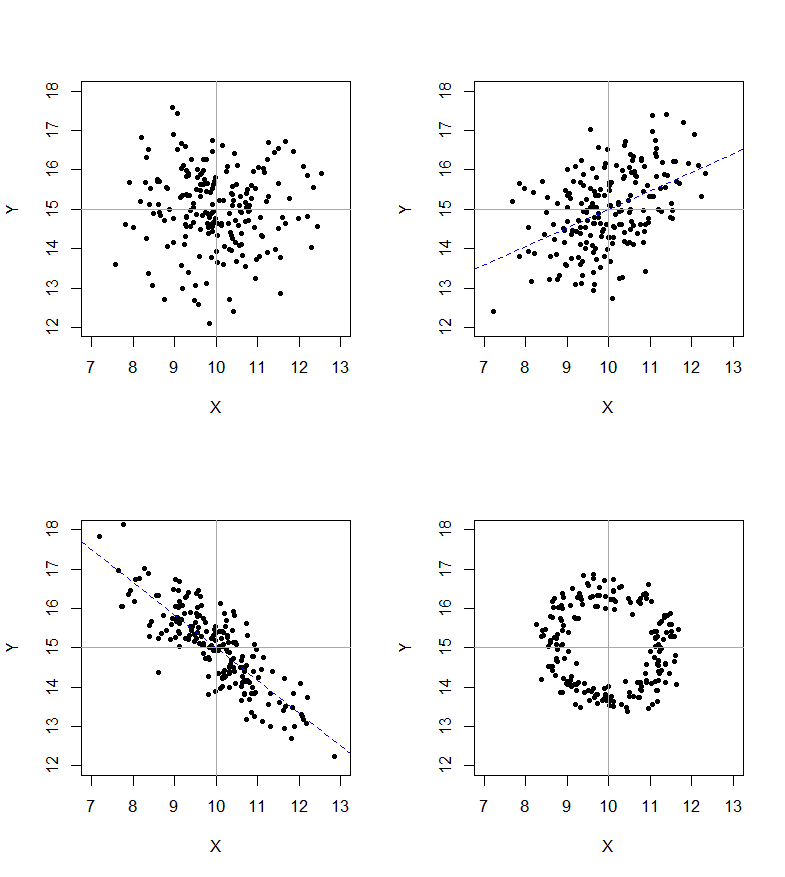
\includegraphics[width=0.7\textwidth]{figures/08-Correlation_linear_regression/scatterplot.png}
        \caption{散佈圖示例}
        \label{fig:scatterplot}
    \end{figure}

    為了量化線性相關的強弱,我們可以將圖\ref{fig:scatterplot}中的每個散佈圖以 $X$ 和 $Y$ 的平均值為基準分成四個象限。可以發現,右上圖呈現正相關,資料點也大多集中在第一和第三象限,也就是兩個變數經常同時大於平均值或同時小於平均值;相對地,左下圖呈現負相關,資料點也大多集中在第二和第四象限,也就是一個變數大於平均值時,另一個變數就常小於平均值,反之亦然;左上和右下兩個散佈圖的資料點則十分均勻地分布在四個象限中。根據這個觀察,我們可以建構以下關於 $X$ 和 $Y$ 的母體參數:
    \[cov(X,Y) = \EE[(X-\mu_X)(Y-\mu_Y)]\]
    其中 $\mu_X := \EE X$ 和 $\mu_Y := \EE Y$ 分別是 $X$ 和 $Y$ 的平均值。可以看到這個量是把 $X$ 和 $Y$ 都中心化(減去平均值)後相乘並取期望值,因此其為正代表 $X$ 和 $Y$ 經常同時大於平均值或同時小於平均值,即正相關;反之,其為負代表 $X$ 和 $Y$ 經常一個大於平均值、一個小於平均值,即負相關。由於這個量可以用來量化兩個隨機變數共同變化的狀況,因此被稱為 $X$ 和 $Y$ 的 \textit{共變異數} 或 \textit{共變數} (covariance)。當共變異數為正時,代表兩個變數呈現正相關;反之則為負相關;若共變異數恰好等於零,則兩個變數沒有線性相關。
    
    根據共變數的定義以及期望值的運算規則,我們可以推出一些以下的性質:
    \allowdisplaybreaks
    \begin{align*}
        cov(X,X) &= \EE[(X - \mu_X)^2] \\
        &= var(X)\\
        cov(X,Y+Z) &= \EE[(X - \EE X)((Y+Z) - \EE(Y+Z))] \\
        &= \EE[(X - \EE X)((Y+Z) - (\EE Y + \EE Z))] \\
        &= \EE[(X - \EE X)((Y-\EE Y) + (Z - \EE Z))] \\
        &= \EE[(X - \EE X)(Y-\EE Y)] + \EE[(X - \EE X)(Z - \EE Z))]\\
        &= cov(X,Y) + cov(X,Z)\\
        cov(aX,bY) &= \EE[(aX-\EE(aX))(bY-\EE(bY))]\\
        &= \EE[(aX-a\EE X)(bY-b \EE Y)]\\
        &= ab \cdot \EE[(X-\EE X)(Y- \EE Y)]\\
        &= ab \cdot cov(X,Y)
    \end{align*}
    第一個性質說明,隨機變數自己和自己的共變異數,等於其變異數。第二個性質顯示共變異數具有分配律。第三個性質則暗示共變異數的數值大小和 $X$ 及 $Y$ 的測量尺度有關:如果原本以公分測量身高、公斤測量體重得到的共變異數為 $4$(公分-公斤),那麼改用公尺測量身高時,身高的數值會變為原本的 $\frac{1}{100}$,而共變異數也會同時變成 $4 \cdot \frac{1}{100} = 0.04$ (公尺-公斤)。換言之,如果使用共變異數來量化身高和體重的線性相關,雖然正負號總會是正的,但其數值大小會隨著測量的單位而變化,而身高和體重的相關性顯然不會因為測量單位不同而有所不同。因此,共變異數不具有尺度不變性 (scale invariance),而非量化線性相關性的良好選擇。

    為了讓相關性的度量不受測量單位所影響,我們可以將中心化的隨機變數用其標準差\textit{標準化}(standardize)後再行相乘,也就是:
    \[\rho_{XY} = \EE\Big[\Big(\frac{X - \mu_X}{\sigma_X}\Big)\Big(\frac{Y - \mu_Y}{\sigma_Y}\Big)\Big] = \frac{cov(X,Y)}{\sigma_X \sigma_Y}\]
    其中 $\sigma_X$ 和 $\sigma_Y$ 為 $X$ 和 $Y$ 的標準差。此時,若 $X$ 因更改測量單位而數值變成 $a$ 倍,則 $X$、$\mu_X$ 和 $\sigma_X$ 均會同時變為 $a$ 倍,使倍數互相抵銷而 $\rho_{XY}$ 不變。這個用以兩個變數相關性的參數,其概念起先由統計學家 Francis Galton 提出,而後其門生 Karl Pearson 詳細推導其統計性質,因而被稱為\textit{皮爾森相關係數} (Pearson correlation coefficient) 或 \textit{皮爾森積差相關係數} (Pearson product-moment correlation coefficient)。皮爾森相關係數除了有我們前面提到的尺度不變性外,根據其定義還能推導出\textbf{其取值範圍為 $-1$ 到 $1$}。其中取值為 $1$ 或 $-1$ 時代表兩個隨機變數互為線性關係(例如 $X = 2Y+3$ 或 $X = -0.3Y-5$),若畫成散佈圖則資料點會呈現完美的直線,此時稱兩個隨機變數為\textit{完全相關} (perfectly correlated)。取值靠近 $1$(或 $-1$)時稱為高度相關,取值靠近 $0$ 時稱為低度相關,取值等於 $0$ 時稱為無線性相關。
    
    由於 $\rho_{XY}$ 是一個母體參數,我們通常仍需要用樣本來估計之,以利進一步對其作統計推論。分母的 $\sigma_X$ 和 $\sigma_Y$ 可以用樣本標準差 $s_X$ 和 $s_Y$ 來估計,分子的共變異數則利用樣本共變異數來估計:
    \[\widehat{cov}(X,Y) = \frac{1}{n-1}\sum_i (X_i - \bar{X})(Y_i - \bar{Y})\]
    其中 $n$ 為樣本數,$\bar{X}$ 和 $\bar{Y}$ 為 $X$ 和 $Y$ 的樣本平均數。這裡分母除以 $n-1$ 的理由和樣本變異數相同,是為了讓樣本共變異數成為母體共變異數的不偏估計量。最終的估計值可以寫為
    \[r_{XY} = \frac{\widehat{cov}(X,Y)}{s_X s_Y} = \frac{\sum_i (X_i - \bar{X})(Y_i - \bar{Y})}{\sqrt{\sum_i (X_i - \bar{X})^2}\sqrt{\sum_i (Y_i - \bar{Y})^2}}\]
    有了 $r_{XY}$ 這個估計值後,除了根據估計值判斷兩個變數的線性相關程度外,也可以針對 $\rho_{XY}$ 進行統計推論。由於 $r_{XY}$ 的抽樣分布通常較為偏斜(尤以 $\rho_{XY}$ 較接近 $-1$ 或 $1$ 時為甚),在進行統計推論前,一般會先對相關係數進行如下的轉換:
    \[z = \frac{1}{2}\ln\Big(\frac{1+r_{XY}}{1-r_{XY}}\Big)\]
    此時假設 $X$ 和 $Y$ 均服從常態分布,則 $z$ 的抽樣分布可用常態分布近似如下:
    \[z \sim \NN\Big(\frac{1}{2}\ln\Big(\frac{1+\rho_{XY}}{1-\rho_{XY}}\Big), \frac{1}{n-3}\Big)\]
    這個轉換方法與近似抽樣分布由統計學家 Ronald Fisher 所提出,因此也被稱為\textit{費雪轉換} (Fisher transformation)。而後即可用此抽樣分布導出 $z$ 在假說檢定中的虛無分佈,或是建構 $\rho_{XY}$ 的信賴區間。其中最常用的是藉由檢定 $\rho_{XY}$ 是否等於零,以推論 $X$ 和 $Y$ 是否有線性相關。然而需要注意的是,兩個變數之間有相關,只代表在資料中他們有朝同一個方向(或相反方向)變動的趨勢,並不代表他們之間必然有因果關係。例如,如果拿每個月的冰淇淋銷量與海邊溺水人數計算相關係數,將會發現有顯著的正相關,但這不代表食用冰淇淋會增加溺水的風險,而只是因為天氣炎熱時同時會讓冰淇淋銷量增加與海邊戲水的人數增加(進而使溺水人數增加),造成兩者數據的同向變化。因此,我們需要利用實驗設計(例如隨機對照實驗)或是排除其他造成相關性的非因果因素,才能將資料中呈現的相關性解釋為因果關係。我們在後續章節談到多重線性回歸時,會再深入探討這個議題,但截至目前為止,讀者應該謹記\textbf{相關不代表因果} (Correlation does not imply causation)。

    \bigskip

    \begin{custom}{練習}
        某研究發現,入住外科加護病房患者的初始體溫(以攝氏度量測)與血清發炎指標 CRP 濃度(以 mg/dL 為單位)之皮爾森相關係數為 0.74。若體溫改為華氏度量測,該相關係數將變為多少?
    \end{custom}

    \bigskip

    \begin{custom}{練習}
        某研究欲了解尿液中的 A 化合物濃度與第二型糖尿病患者的糖化血色素是否有相關。搜集了 103 名病患並計算兩者之相關係數後得到估計值及其 95\% 信賴區間為 0.150 (-0.045, 0.334)。在設定顯著水準為 0.05 下,請根據研究問題進行假說檢定並說明結論。
    \end{custom}

\section{簡單線性回歸}

    我們前一節提到可以用相關係數來描述兩個變數之間的線性關係。舉例而言,如果清華大學學生的身高與體重的相關係數為 0.8,呈現頗強的正相關。這代表身高較高的學生體重也相對較高。然而,這個相關係數只告訴我們兩個變數間呈現正向的線性關係,而不能告訴我們隨著身高的增加,體重\textbf{增加的幅度}為何。另外,我們也不能從相關係數來\textbf{預測}給定身高下,學生體重的預期值為何。由此看來,相關係數只給了我們兩個變數間線性關係的強度和方向,但是並沒有給我們該線性關係的全貌。

    \subsection{簡單線性回歸的模型與參數}
    
    為了瞭解兩個變數 $Y$ 與 $X$ 之間的線性關係,統計上採取的策略是先建立 $Y$ 和 $X$ 之間的線性模型,然後用資料估計模型的參數,並對這些參數來做推論。我們以圖 \ref{fig:SLR} 為例,散佈圖如左圖。假設體重變數記為 $Y$,身高變數記為 $X$,而且我們有興趣的是在身高 $X$ 變化下,體重 $Y$ 的預期變動。此時 $Y$ 稱為\textit{反應變數} (response variable) 或\textit{應變數} (dependent variable),而 $X$ 稱為\textit{解釋變數} (explanatory variable) 或\textit{自變數} (independent variable)。理想上,我們希望可以直接用一條直線 $Y = \beta_0 + \beta_1 X$ 來完全描述 $Y$ 和 $X$ 之間的關係,但大多數情況下兩個變數不會剛好呈現直線關係(除非兩者呈現完全相關)。因此,我們退而求其次,假設
    \[Y = \beta_0 + \beta_1 X + \varepsilon, \qquad \varepsilon \sim \NN(0, \sigma^2)\]
    其中 $\beta_0 + \beta_1 X$ 代表的是圖 \ref{fig:SLR} 左圖的黑色斜直線,也就是給定身高下,模型預期的體重。$\varepsilon$ 則是誤差項,代表實際值和預期值的差異,也就是每個觀察值黑點到斜直線的垂直距離。誤差項的來源可能來自測量誤差,但更多時候是起源於研究中未測量到的變數。例如,如果學生中有一群人偏高熱量飲食、一群人則篇低熱量飲食,我們分別以圖 \ref{fig:SLR}中間和右邊的子圖獨立標記這兩群人後可以發現,考量飲食熱量高低對體重的影響後,同一群飲食習慣者內部的誤差項就相對較小。誤差項的分佈方面,我們假設它們服從平均值為$0$,變異數為 $\sigma^2$ 的常態分布。注意到我們這裡假設不論 $X$ 是多少,誤差項的變異數皆為 $\sigma^2$,這個假設被稱為\textit{同質變異性} (homoscedasticity)。同質變異性的假設不見得在所有資料都成立,例如體重的變異性可能在身高較高的人較大,在身高較矮的人則較小,此時就需要使用較進階的統計方法來處理這類\textit{異質變異性} (heteroscedasticity) 的課題。在這個章解中,為了簡化流程,我們仍然保留同質變異性的假設。

    我們以下回顧整理簡單線性回歸所做的假設,其代表的英文字恰恰可以縮寫成「LINE」:
    \begin{itemize}
        \item 線性(\textbf{L}inearity):給定自變數 $X$ 下,應變數 $Y$ 的期望值和 $X$ 的取值呈線性關係。
        \item 獨立誤差(Error \textbf{I}ndependence):每個觀察值的誤差 $\epsilon_i$ 均互相獨立。
        \item 常態誤差(Error \textbf{N}ormality):每個觀察值的誤差 $\epsilon_i$ 均服從常態分佈。
        \item 同質變異性(Homoscedasticity, 或 Error \textbf{E}quivariance):每個觀察值的誤差 $\epsilon_i$ 變異數均等。
    \end{itemize}
    注意到我們只假設了\textbf{誤差}呈現常態,而對 $Y$ 和 $X$ 的分布並沒有進行限制。換言之,進行簡單線性回歸時,應變數和自變數\textit{不需要}遵從常態分佈。

    \begin{figure}[htbp]
        \centering
        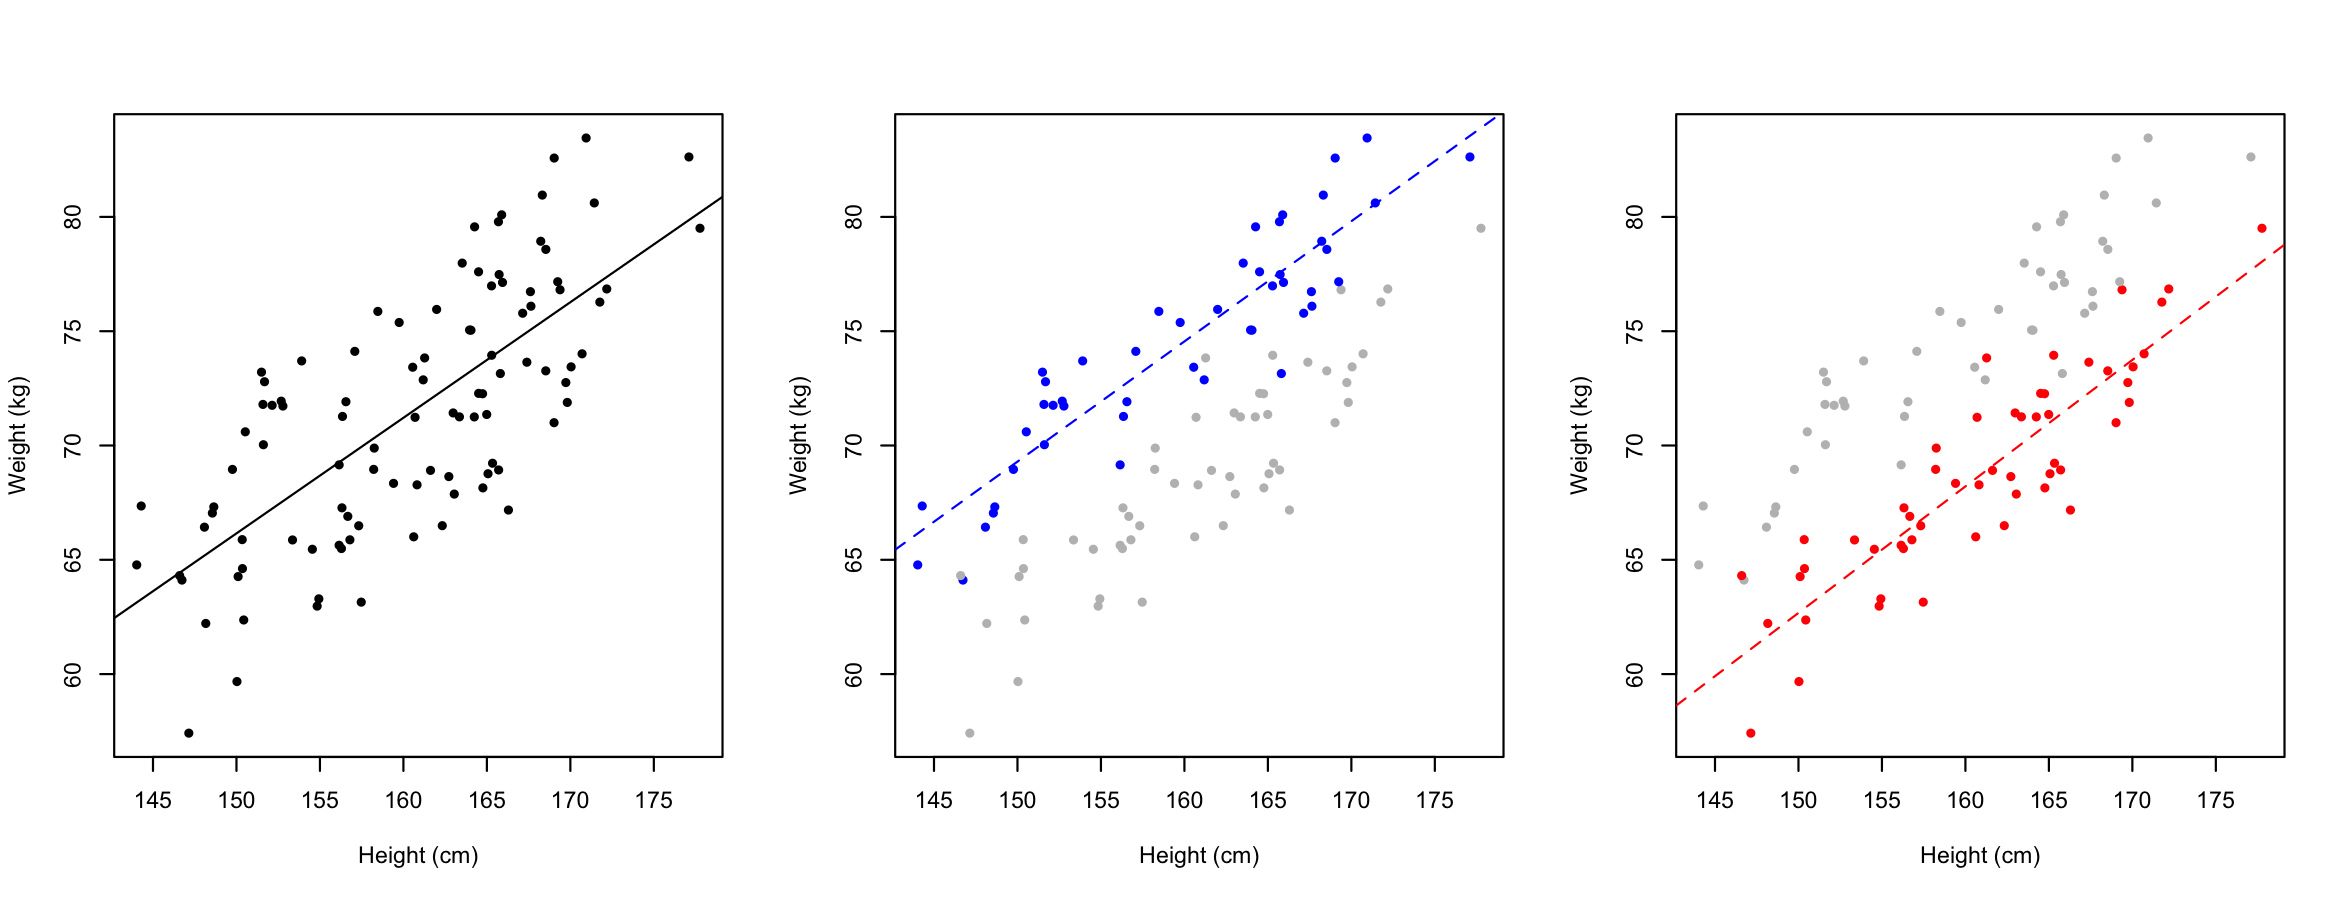
\includegraphics[width=\textwidth]{figures/08-Correlation_linear_regression/regression.png}
        \caption{簡單線性回歸的散佈圖}
        \label{fig:SLR}
    \end{figure}

    根據前述的簡單線性回歸模型,當我們已知一個學生的身高為 $x$ 公分,那麼他的實際體重會以 $\beta_0 + \beta_1 x$ 公斤為中心,加入一個上下變動的誤差項,且這個誤差項來自於變異數為 $\sigma^2$ 的常態分布。我們無法預測誤差項的值,但知道其期望值為零,因此我們預期該學生的身高\textbf{平均而言}為 $\beta_0 + \beta_1 x$ 公斤。準此,我們就能得出模型中兩個參數 $\beta_0, \beta_1$ 的白話解釋(這兩個係數又被稱為\textit{回歸係數} (regression coefficients))
    \begin{itemize}
        \item $\beta_0$:又被稱為\textit{截距} (intercept),代表解釋變數 $X$ 取值為 $0$ 時,反應變數 $Y$ 的平均值。
        \item $\beta_1$:又被稱為\textit{斜率} (slope),代表解釋變數 $X$ 每增加 $1$ 單位時,反應變數 $Y$ 的平均值的增加量。
    \end{itemize}
    可以看出,通常我們有興趣的是斜率 $\beta_1$:當 $\beta_1 \ne 0$ 時,代表解釋變數 $X$ 的變動對於反應變數 $Y$ 有線性影響。至於截距 $\beta_0$ 的數值我們通常不太關心,這個數值甚或不符合現實情境。例如在上述的例子中,$\beta_0$ 代表一個 $0$ 公分的學生預期的平均體重。這在現實上沒有任何實用意義,只是回歸模型外插至 $X=0$ 用以建模的參數而已。

    \subsection{簡單線性回歸的參數估計及推論}

    建立線性回歸模型後,我們的目的是要利用資料估計模型的參數並進行推論。假設我們把第 $i$ 個觀察值的反應變數和解釋變數數值記為 $Y_i$ 和 $X_i$。另外,我們將斜率的估計值寫為 $\hat{\beta}_1$、截距的估計值寫為 $\hat{\beta}_0$,那麼對於第 $i$ 個觀察值,我們預期其反應變數的平均值為 $\hat{\beta}_0 + \hat{\beta}_1 X_i$,而其反應變數的實際數值為 $Y_i$。這兩者之間的差 $e_i = Y_i - (\hat{\beta}_0 + \hat{\beta}_1 X_i)$ 被稱為 \textit{殘差} (residual)。殘差的大小越小,代表我們的估計越準,因此我們目標應該要將總體的殘差大小最小化。在統計中,為了計算方便,我們最小化的是每個觀察值的殘差平方的總和,如下所示。這個方法也被稱為\textit{最小平方法} (method of least squares):
    \[L = \sum_i e_i^2 = \sum_i  [Y_i - (\hat{\beta}_0 + \hat{\beta}_1 X_i)]^2\]
    利用簡單的微分(或是二次多項式求極值的方法)可得,能夠將 $L$ 最小化的 $\hat{\beta}_1$ 和 $\hat{\beta}_0$ 為
    \begin{align*}
        \hat{\beta}_1 &= \frac{\sum_i (X_i - \bar{X})(Y_i - \bar{Y})}{\sum_i (X_i-\bar{X})^2} = \frac{\widehat{cov}(X,Y)}{s_X^2} = r_{XY}\frac{s_Y}{s_X}\\
        \hat{\beta}_0 &= \bar{Y} - \hat{\beta_1}\bar{X}
    \end{align*}
    注意到 $\hat{\beta}_1$ 恰好等於 $r_{XY}$ 乘上一個恆正的 $s_Y / s_X$,因此他們的正負號是同向的。這很符合直覺,因為當兩個變數呈現正相關時,我們預期其中一個變數增加時,另一個變數也會同時增加,因此回歸斜率為正;反之當呈現負相關時,兩個變數的增減趨勢相反,所以回歸斜率應為負。為了進一步了解這組估計值的好壞,我們可以計算 $\hat{\beta}_1$ 和 $\hat{\beta}_0$ 的期望值和變異數,並得到
    \begin{align*}
        \EE\hat{\beta}_1 = \beta_1 \quad &; \quad \EE\hat{\beta}_0 = \beta_0\\
        var(\hat{\beta}_1) = \frac{\sigma^2}{(n-1)s_X^2} \quad &; \quad var(\hat{\beta}_0) = \sigma^2\Big(\frac{1}{n} + \frac{\bar{X}^2}{(n-1)s_X^2}\Big)
    \end{align*}
    首先我們可以看到這兩個估計值都是\textbf{不偏}的,也就是說它們的期望值都恰好等於他們要估計的母體參數 $\beta_1$ 和 $\beta_0$。另外關於估計值變異數的部分,我們可以分成幾個影響因子來看:
    \begin{itemize}
        \item 誤差的母體變異數 $\sigma^2$:由於誤差代表資料中無法被回歸模型解釋的部分,因此誤差變異數越大,代表資料中能用來推論回歸模型的資訊越少。因此,兩個回歸係數的估計值變異數都正比於誤差變異數,代表資料資訊越少,回歸係數估計值的準確度越低。
        \item 樣本數 $n$:樣本數增大,資料的資訊也增加,因此估計值變異數均會變小。
        \item 解釋變數的樣本變異數 $s_X^2$:當解釋變數變異數變小,代表資料中解釋變數的跨度較小,此時只要資料稍有變動,對於斜率的估計就會變化得很劇烈。讀者可以把回歸線想像成一根擀麵棍:當解釋變數跨度很大時,就像用雙手十隻手指分散地握住桿麵棍,即便其中一隻手指頭出力,桿麵棍也不會明顯地歪斜。相對地,解釋變數跨度很小時,就像雙手的手指擠在桿麵棍的中央,此時只要其中一根手指稍微出力,其他手指很難抗衡其變化,桿麵棍就會歪斜。
    \end{itemize}
    取得回歸係數的估計值後,注意到 $\hat{\beta}_1$ 和 $\hat{\beta}_0$ 的變異數都含有 $\sigma^2$,但 $\sigma^2$ 目前未知仍待估計。根據模型的假設,第 $i$ 個觀察值的誤差 $\varepsilon_i$ 可以移項寫成
    \[\varepsilon_i = Y_i - (\beta_0 + \beta_1 X_i) \sim \NN(0, \sigma^2)\]
    雖然我們不知道實際的誤差$\varepsilon_i$,但我們可以用殘差 $e_i = Y_i - (\hat{\beta}_0 + \hat{\beta}_1 X_i)$ 來估計誤差 $\varepsilon_i$,進而用殘差的「樣本變異數」來估計誤差的母體變異數 $\sigma^2$
    \[\hat{\sigma}^2 = \frac{1}{n-2}\sum_i e_i^2 = \frac{1}{n-2}\sum_i [Y_i - (\hat{\beta}_0 + \hat{\beta}_1 X_i)]^2\]
    這裡的樣本變異數和一般的樣本變異數公式有點差別:(1) 分母的部分不是 $n-1$ 而是 $n-2$,因為在計算時我們使用了 \textbf{2} 個估計的參數 $\hat{\beta}_1$ 和 $\hat{\beta}_0$,因此自由度要扣掉 $2$(一般的樣本變異數只使用了一個估計的參數 $\bar{X}$),(2) 平方和的部分 $e_i$ 沒有減去樣本平均,因為我們已知誤差的期望值為 $0$。取得誤差變異數的估計值 $\hat{\sigma}^2$ 後,我們就可以用資料估計出回歸係數估計值的變異數如下:
    \[\widehat{var}(\hat{\beta}_1) = \frac{\widehat{\sigma}^2}{(n-1)s_X^2} \quad ; \quad \widehat{var}(\hat{\beta}_0) = \hat{\sigma}^2\Big(\frac{1}{n} + \frac{\bar{X}^2}{(n-1)s_X^2}\Big)\]
    我們更常報告的是標準誤,也就是將變異數估計值開根號:
    \[\widehat{se}(\hat{\beta}_1) = \sqrt{\frac{\widehat{\sigma}^2}{(n-1)s_X^2}} \quad ; \quad \widehat{se}(\hat{\beta}_0) = \sqrt{\hat{\sigma}^2\Big(\frac{1}{n} + \frac{\bar{X}^2}{(n-1)s_X^2}\Big)}\]

    取得回歸係數的估計值以及其變異數後,我們就能對回歸係數進行假說檢定或是建立信賴區間。此處我們需要借助 $t$ 分布,並且有:
    \[\frac{\hat{\beta}_1-\beta_1}{\widehat{se}(\hat{\beta}_1)} \sim t_{n-2} \quad ; \quad \frac{\hat{\beta}_0-\beta_0}{\widehat{se}(\hat{\beta}_0)} \sim t_{n-2}\]
    此處 $t$ 分布的自由度為 $n-2$,同樣是因為計算分母的標準誤估計值時使用了兩個參數估計值。同理於前幾章的 $t$ 檢定,如果要進行顯著水準設定為 $\alpha$、假說為 $H_0: \beta_1 = 0;\; H_1: \beta_1 \ne 0$ 的雙尾檢定,則可計算 $t$ 檢定統計量(虛無假說下 $\beta_1 = 0$):
    \[t = \frac{\hat{\beta}_1}{\widehat{se}(\hat{\beta}_1)}\]
    該檢定的 $p$ 值即為 $2\times\PP(t_{n-2} \ge |t|)$,檢定統計量的拒絕區則為 $|t| \ge t_{n-2, \alpha/2}$。相對地,如果要建構 $\beta_1$ 的 $(1-\alpha)\times 100\%$ 雙尾信賴區間,則為:
    \[\Big(\hat{\beta}_1 - t_{n-2, \alpha/2}\widehat{se}(\hat{\beta}_1), \hat{\beta}_1 + t_{n-2, \alpha/2}\widehat{se}(\hat{\beta}_1)\Big)\]
    關於 $\beta_0$ 的假說檢定和信賴區間建構和 $\beta_1$ 相同,只是如同我們之前所說,大多數的時候我們對截距的推論不感興趣。事實上,一般在研究中甚至不會報告截距的估計值、信賴區間以及檢定結果。

    在簡單線性回歸中,我們還可以探討一個特例:如果自變數 $X$ 為二元變項且取值為 $0$ 或 $1$,代表觀察值可以被分成兩組,一組為 $X=0$、一組為 $X=1$。根據簡單線性回歸的模型假設:
    \[Y = \left\{\begin{array}{lr}
        \beta_0 + \varepsilon, & X = 0\\
        \beta_0 + \beta_1 + \epsilon, & X = 1
    \end{array}, \qquad \varepsilon \sim \NN(0, \sigma^2) \right.\]
    該假設顯示,$X=0$ 這一組的 $Y$ 母體平均為 $\beta_0$,$X=1$ 這一組的 $Y$ 母體平均為 $\beta_0 + \beta_1$,而且各組內部的觀察值都服從變異數為 $\sigma^2$ 的常態分布。因此,我們也可以把上述模型假設寫成:
    \[\left\{\begin{array}{lr}
        Y \sim \NN(\beta_0,\sigma^2), & X = 0\\
        Y \sim \NN(\beta_0 + \beta_1, \sigma^2), & X = 1
    \end{array} \right.\]
    可以發現,這組假設和「假設兩組母體變異數相等」的獨立樣本 $t$ 檢定所做的假設完全等價,而獨立樣本 $t$ 檢定之檢定標的是兩組母體平均的差,恰好就是 $\beta_1$。因此,針對兩組獨立資料,進行獨立樣本 $t$ 檢定會等同於檢定「以組別編碼 $X=0,1$ 為自變數的線性回歸斜率」。

    \bigskip

    \begin{custom}{練習}
       某研究將 HIV 病患血液中「CD4$^+$ T 細胞的個數對數 (以 10 為底)」對「接受抗病毒治療與否(接受 = 1、未接受 = 0)」作簡單線性回歸,得到斜率估計值與雙尾 $95\%$ 信賴區間為 $0.301$ 及 $(0.176,0.426)$。請用白話說明該回歸模型之結果。
    \end{custom}

    \bigskip

    \begin{custom}{思考}
       如果將體重(公斤)對身高建立兩個線性回歸模型,一個模型的身高用公分作單位,另一個模型的身高用公尺作單位,得到結果如下:

       \medskip
       
       \begin{tabular}{cccccccc}
            \toprule
            \multirow{2}{*}{身高單位} & \multicolumn{3}{c}{斜率} && \multicolumn{3}{c}{截距} \\
            \cline{2-4}\cline{6-8}
            & 估計值 & 標準誤 & 雙尾 $p$ 值 && 估計值 & 標準誤 & 雙尾 $p$ 值\\
            \hline
            公分 & $\hat{\beta}_1$ & $\hat{s}_1$ & $p_1$ && $\hat{\beta}_0$ & $\hat{s}_0$ & $p_0$ \\  
            公尺 & $\hat{\beta}_1^*$ & $\hat{s}_1^*$ & $p_1^*$ && $\hat{\beta}_0^*$ & $\hat{s}_0^*$ & $p_0^*$ \\
            \bottomrule
       \end{tabular}

       \medskip

       \noindent 請問每個 column 的兩個數值(例如 $\hat{\beta}_1$ 和 $\hat{\beta}_1^*$)的關係為何?
    \end{custom}

    \bigskip

    \begin{custom}{思考}
       前面我們提到,回歸係數 $\beta_1$ 的意義為「解釋變數 $X$ 每增加一單位,反應變數 $Y$ 平均增加的單位數」。後來我們推導出,$\beta_1$ 的估計值 $\hat{\beta}_1$ 和相關係數 $\rho_{XY}$ 的估計值 $r_{XY}$ 的關係為 $\hat{\beta}_1 = r_{XY} \frac{s_Y}{s_X}$。事實上,$\beta_1$ 和 $\rho_{XY}$ 的亦有相似的關係:
       \[\beta_1 = \rho_{XY} \frac{\sigma_Y}{\sigma_X} \qquad \; \qquad \rho_{XY} = \beta_1 \frac{\sigma_X}{\sigma_Y}\]
       其中 $\sigma_Y, \sigma_X$ 分別為 $Y$ 和 $X$ 的母體標準差。根據這個定義, $\rho_{XY}$ 的解釋意義為何?由於 $\rho_{XY}$ 必定介於 $-1$ 與 $1$ 之間,讀者是否能想像 Francis Galton 當初在發展回歸理論時,為何要將它稱之為「回歸 (regression)」?
    \end{custom}
    
    \section{簡單線性回歸模型的模型配適度與模型診斷}

    在配適完線性回歸模型後,除了檢視回歸係數的估計值以及統計推論結果外,我們也常想知道配適出的模型是否能有效地預測反應變數。在線性回歸中,模型的解釋力常以「解釋的變異比例」來量化。我們可以再次回到圖\ref{fig:SLR}關於預測體重的散布圖,並考慮兩種可能的預測模型:僅有身高、以及同時有身高和飲食習慣。資料中體重的分布寬度大約是 20 公斤。當我們用身高去預測體重,每個人的體重扣掉預測值後(即殘差),分布寬度就減小到約 10 公斤。如果我們進一步同時用身高和飲食習慣來預測體重,殘差的分布寬度更減低到 5 公斤左右。我們可以看到,隨著模型的解釋力越來越好,殘差的變異性、也就是模型未能解釋的資料變異性越來越小。我們可以把上述的觀察用下面的式子具象化:
    \[\text{總變異}  = \text{模型解釋變異} + \text{殘差變異}\]
    在線性回歸中,我們會用各種\textit{平方和} (sum of squares)來描述上面三項變異:
    \begin{itemize}
        \item 總變異:\textit{總平方和}(total sum of squares, SST)$\sum_i (Y_i - \bar{Y})^2$,描述資料相對於總平均的偏差。
        \item 模型解釋變異:\textit{回歸平方和} (regression sum of squares, SSR)$\sum_i (\hat{Y}_i - \bar{Y})^2$,描述模型預測值 $\hat{Y}_i$相對於總平均的偏差。
        \item 殘差變異:\textit{殘差平方和}(residual (error) sum of squares, SSE)$\sum_i (Y_i - \hat{Y}_i)^2$,描述資料相對於預測值的偏差。
    \end{itemize}
    這些平方和的定義恰好可以滿足我們上面的式子:
    \[\underbrace{\sum_i (Y_i - \bar{Y})^2}_{SST} = \underbrace{\sum_i (\hat{Y}_i - \bar{Y})^2}_{SSR} + \underbrace{\sum_i (Y_i - \hat{Y}_i)^2}_{SSE}\]
    從這個式子可以看到,藉由配適模型得到預測值 $\hat{Y}$,可以將總變異(SST)分割為模型可解釋的變異(SSR)和模型不能解釋的變異(SSE)兩個部分。我們可以將模型的解釋力用 SSR 和 SST 的比值 SSR/SST、也就是\textbf{模型解釋的變異比例}來代表。這個值被稱為模型的\textit{決定係數} (coefficient of determination) $R^2$,其取值範圍為 $0$ 到 $1$(因 SSR 和 SSE 均非負),越靠近 $1$ 代表模型的解釋力越強。實際將 $R^2$ 的計算方法寫出來可以發現:
    \begin{align*}
        R^2 = \frac{SSR}{SST} &= \frac{\sum_i (\hat{Y}_i-\bar{Y})^2}{\sum_i (Y_i - \bar{Y})^2}\\
        &= \frac{\sum_i (\hat{\beta}_0 + \hat{\beta}_1 X_i -\bar{Y})^2}{\sum_i (Y_i - \bar{Y})^2}\\
        &= \frac{\sum_i (\bar{Y} - \hat{\beta}_1 \bar{X}+ \hat{\beta}_1 X_i -\bar{Y})^2}{\sum_i (Y_i - \bar{Y})^2}\\
        &= \hat{\beta}_1^2 \frac{\sum_i (X_i - \bar{X})^2}{\sum_i (Y_i - \bar{Y})^2}\\
        &= \Big(\frac{\sum_i (X_i-\bar{X})(Y_i-\bar{Y})}{\sum_i (X_i-\bar{X})^2}\Big)^2 \frac{\sum_i (X_i - \bar{X})^2}{\sum_i (Y_i - \bar{Y})^2} \\
        &= \frac{[\sum_i (X_i-\bar{X})(Y_i-\bar{Y})]^2}{\sum_i (X_i - \bar{X})^2\sum_i (Y_i - \bar{Y})^2} = r_{XY}^2
    \end{align*}
    因此,\textbf{簡單線性回歸的決定係數恰為皮爾森相關係數的平方}。皮爾森相關係數越靠近 $1$ 或 $-1$,代表兩個變數的線性相關程度越強,也代表配適簡單線性回歸時的模型解釋力越大。

    最後,在配適線性回歸模型時,我們做了四個重要的模型假設:線性、獨立誤差、常態誤差、同質變異性,而我們的統計推論正確與否也取決於這些模型假設是否正確。因此,在取信於模型的推論前,我們應該先確認模型的假設是否符合資料,這個程序被稱為\textit{模型診斷}(model diagnostics)。針對線性的假設部分,我們可以用散布圖來觀察兩個變數間的關係是否為線性,獨立誤差的部分則可以用資料搜集的過程來論證。不過常態誤差和同質變異性的假設,則因為是針對誤差而非資料的觀察值,我們必須利用殘差來做圖分析。圖\ref{fig:diagnostics}的左上、右上和左下三個圖是拿回歸的殘差對自變數 $X$ 作圖。殘差是誤差的估計值,而根據假設,誤差應該不論 $X$ 取值為何均服從相同變異數的常態分配。因此,正常的殘差圖應該如左上角,顯示殘差的分布不論 $X$ 取值為何均相同。右上角中,明顯看到殘差和 $X$ 仍然有一個曲線關係,這隱含著線性假設被違反。左下角中,殘差的變異數隨著 $X$ 增大而增大,隱含著同質變異性假設被違反。針對常態性假設,則可以繪製如右下角的常態百分位-百分位圖(或稱為\textit{常態 QQ 圖} (normal QQ plot))。在 QQ 圖中,每個點代表一個殘差值,橫坐標代表該殘差如果來自標準常態分布,根據其百分位數應該要取值多少(例如第 95 百分位應該取值 1.96):縱座標則為其實際取值。如果殘差的分布呈現常態,則這些殘差點應該會呈現一個左下到右上的直線,如右下圖的虛線所示。如果 QQ 圖顯示的圖形並非左下到右上的直線,則暗示著常態性假設有待商榷。前述模型診斷的結果如果顯示假設被違反,我們就需要回頭過來修改模型,例如進行非線性的回歸,或是套用更進階的統計方法來處理非常態或異質性的的誤差。

    \begin{figure}[htbp]
        \centering
        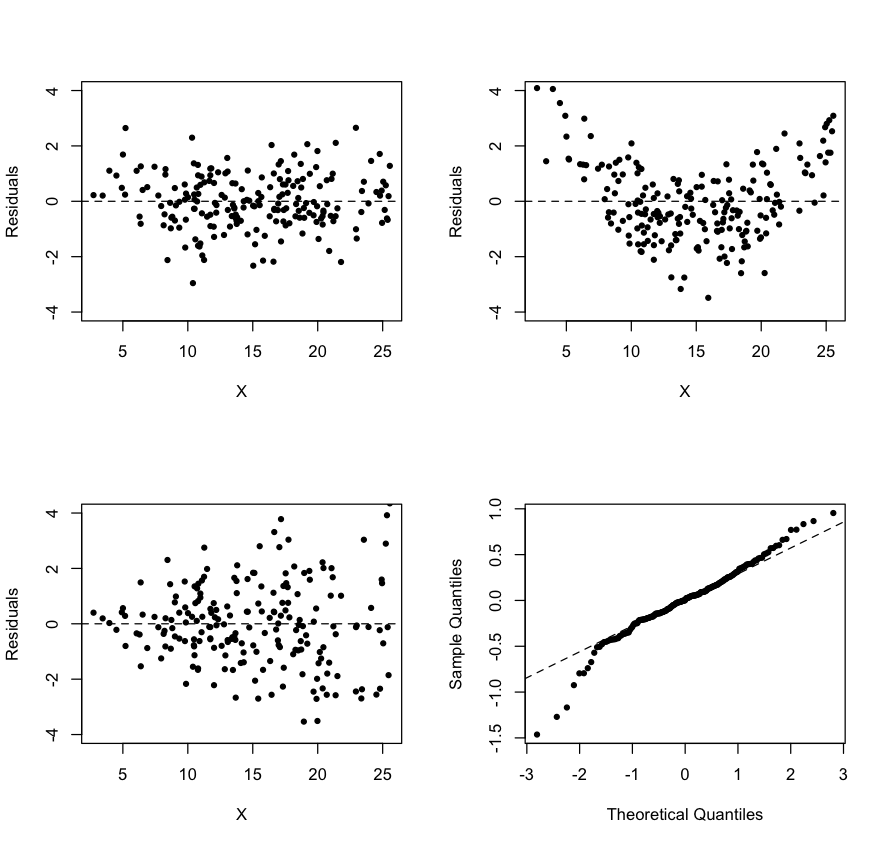
\includegraphics[width=\textwidth]{figures/08-Correlation_linear_regression/diagnostics.png}
        \caption{殘差圖與殘差 QQ 圖}
        \label{fig:diagnostics}
    \end{figure}

\section{多重線性回歸}
    在前面的章節中,我們使用簡單線性回歸來探討一個解釋變數 $X$ 和一個反應變數 $Y$ 的關係,但在生物醫學研究中,影響反應變數 $Y$ 的解釋變數往往不只一個。例如在圖\ref{fig:SLR}的例子中,一個人的體重可能與他的身高和飲食習慣均有關係。此時我們希望能在回歸模型中同時加入多個解釋變數,以增進模型對反應變數的解釋力。這種有多個解釋變數的線性模型被稱為\textit{多重線性回歸} (multiple linear regression),或簡稱多重回歸。

    假設我們有興趣的反應變數是 $Y$,另外有 $p$ 個用來解釋 $Y$ 的變數 $X_1, X_2, X_3,..., X_p$。多重線性回歸的模型假設如下:
    \[Y = \beta_0 + \beta_1 X_1 + \beta_2 X_2 + \cdots + \beta_p X_p + \varepsilon, \qquad \varepsilon \sim \NN(0,\sigma^2)\]
    可以看到多重線性回歸同樣繼承了簡單線性回歸的四個假設:(1) 線性:給定解釋變數下,$Y$ 的期望值是這些變數的線性組合 (2) 獨立誤差:每筆觀察值的誤差 $\varepsilon_i$ 均獨立 (3) 常態誤差:誤差均服從常態分布 (4) 同質變異性:誤差變異數不隨解釋變數取值而變化。
    
    上述多重線性回歸模型中,截距項 $\beta_0$ 的解釋意義和簡單線性回歸類似:當所有的解釋變數都取值為 $0$ 時,$Y$ 的平均值即為 $\beta_0$。至於其他回歸係數,例如 $\beta_1$ 的意義,則是在 \textit{控制其他解釋變數不變的情況下},$X_1$ 每增加 $1$ 單位時,$Y$ 平均值的變化。這裡之所以需要強調控制其他解釋變數不變,是因為各解釋變數經常會有相關性,因此其中一個解釋變數變動時,可能隱含了其他變數也會有預期下的變動。舉例來說,如果身高和體重均為解釋變數,那麼我們在想像一個身高較高的人時,其實也預期其體重也會較重。然而,身高的回歸係數說明的是,在\textbf{同樣體重}的情況下,身高每增加一單位,反應變數平均值的變化。

    \begin{figure}[htbp]
        \centering
        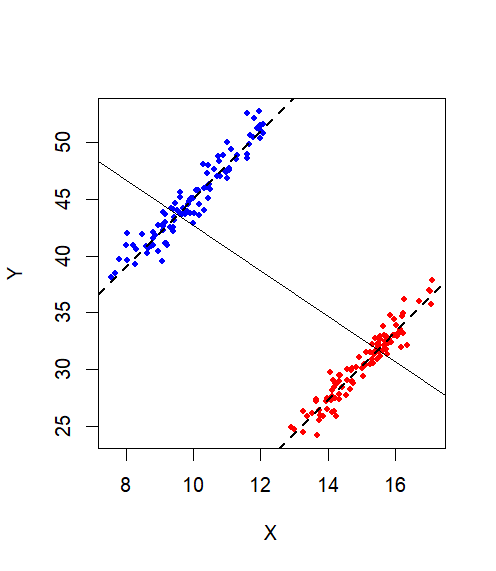
\includegraphics[width=0.5\textwidth]{figures/08-Correlation_linear_regression/confounding.png}
        \caption{多重回歸和簡單回歸結論不同的演示}
        \label{fig:confounding}
    \end{figure}
    
    多重回歸這個「控制其他解釋變數」的特性,甚至可能造成簡單回歸和多重回歸關於變數關係的方向結論不同。如圖\ref{fig:confounding}的散布圖所示,假設我們想知道變數 $X$ 與變數 $Y$ 的關係。直接將 $Y$ 對 $X$ 進行簡單回歸會得到黑色的回歸線。其斜率為負,亦即隨著 $X$ 的取值增加,$Y$ 的平均值會降低。然而,如果我們還知道每個觀察值可以分為紅色和藍色兩組,並把組別編碼為一個二元變數 $Z$ 後,將 $Y$ 對 $X$ 和 $Z$ 進行多重回歸,此時 $X$ 的回歸係數代表\textbf{控制顏色變數 $Z$ 不變的情況下},$X$ 每增加一單位,$Y$ 的平均增加量。從圖中可以看出,不論是控制顏色組別為藍色或紅色,$Y$ 的平均反而都是隨著 $X$ 增加而增加,和簡單回歸的結論不同。
    
    不過注意到,上面簡單回歸和多重回歸的結論雖然不同,但兩者\textbf{都是正確的}:如果僅從 $X$ 的數值想單方向地預測 $Y$,那麼較大的 $X$ 的確應該預測出較低的 $Y$。然而控制顏色組別 $Z$ 的影響後,$X$ 和 $Y$ 的關係就轉變為正向。這種新增解釋變數後造成回歸係數方向相反的現象也被統計學家稱為\textit{逆轉悖論} (reversal paradox)。

    多重線性回歸的回歸係數依然最常以最小平方法來估計,但計算的過程牽涉到矩陣運算,因此在這裡我們不會深入探討。獲得回歸係數的估計值 $\hat{\beta}_0, \hat{\beta}_1, \hat{\beta}_2, ... \hat{\beta}_p$後,即可依類似簡單線性回歸的方法計算各觀察值的殘差:
    \[e_i = Y_i - (\hat{\beta}_0 + \hat{\beta}_1 X_i + \hat{\beta}_2 X_2 + \cdots + \hat{\beta}_p X_p)\]
    而殘差的「樣本變異數」即為誤差變異數的估計值:
    \[\hat{\sigma}^2 = \frac{1}{n-p-1}\sum_i e_i^2\]
    注意到這裡的分母和簡單線性回歸不同,因為計算殘差時用到 $p+1$ 個回歸係數估計值,所以分母的地方要減去 $p+1$。得到誤差變異數的估計值後,即可再經過矩陣運算得到各回歸係數估計值 $\hat{\beta}_0, \hat{\beta}_1, \hat{\beta}_2, ... \hat{\beta}_p$ 的標準誤估計值 $\widehat{se}(\hat{\beta}_0), \widehat{se}(\hat{\beta}_1), \widehat{se}(\hat{\beta}_2), ..., \widehat{se}(\hat{\beta}_p)$。

    利用回歸係數的估計值及其標準誤的估計值,即可對各迴歸係數進行假說檢定或信賴區間的建構。我們同樣借助 $t$ 分布,並且有:
    \[\frac{\hat{\beta}_j - \beta_j}{\widehat{se}(\hat{\beta}_j)} \sim t_{n-p-1}, \qquad j = 0,1,2,...p\]
    此處 $t$ 分布的自由度為 $n-p-1$,因為計算分母的標準誤估計值時使用了 $p+1$ 個參數估計值。和簡單回歸同理,如果要進行顯著水準為 $\alpha$,檢定 $\beta_j$ 是否為 $0$ 的雙尾檢定,則可計算如下 $t$ 檢定統計量:
    \[t = \frac{\hat{\beta}_j}{\widehat{se}(\hat{\beta}_j)}\]
    該檢定的 $p$ 值為 $2\times\PP(t_{n-p-1} \ge |t|)$,檢定統計量的拒絕區則為 $|t| \ge t_{n-p-1, \alpha/2}$。當虛無假說被拒絕時,代表在控制其他解釋變數不變的情況下,解釋變數 $X_j$ 和 $Y$ 之間有顯著的線性關係。如果要建構 $\beta_j$ 的 $(1-\alpha)\times 100\%$ 雙尾信賴區間,則為:
    \[\Big(\hat{\beta}_j - t_{n-p-1, \alpha/2}\widehat{se}(\hat{\beta}_j), \hat{\beta}_j + t_{n-p-1, \alpha/2}\widehat{se}(\hat{\beta}_j)\Big)\]
    
\section{多重線性回歸的模型選擇}
    在多重線性回歸中,除了檢定其中一個回歸係數是否為 $0$ 外,有時候我們有興趣的命題是一群回歸係數是否同時為 $0$。例如(不失一般性地)我們想知道 $\beta_1, \beta_2, ..., \beta_q$ 是否同時為零,此時我們的假說可寫為:
    \[\left\{\begin{array}{l}
        H_0: \beta_1 = \beta_2 = \cdots = \beta_q = 0\\
        H_1: (\beta_1 \ne 0) \text{ or } (\beta_2 \ne 0) \text{ or } ... \text{ or } (\beta_q \ne 0)
    \end{array}\right.\]
    在虛無假說 $H_0$ 下,$\beta_1, \beta_2, ..., \beta_q$ 均為 $0$,意味著我們在配適多重線性回歸時,其實不用納入 $X_1, X_2, ..., X_q$,只要納入 $X_{q+1}, X_{q+2}, ..., X_p$ 即可。我們可以把這個比較限縮的模型稱為 $M_0$(意味著虛無假說下的模型),而將納入所有解釋變數的模型稱為 $M_1$(意味著對立假說下的模型),整理如下:
    \[\left\{\begin{array}{ll}
        M_0: Y = \beta_0  &+ \beta_{q+1} X_{q+1} + \beta_{q+2} X_{q+2} + \cdots + \beta_{p} X_{p} + \varepsilon\\
        M_1: Y = \beta_0 + \beta_1 X_1 + \beta_2 X_2 + \cdots  + \beta_q X_q &+ \beta_{q+1} X_{q+1} + \beta_{q+2} X_{q+2} + \cdots + \beta_{p} X_{p} + \varepsilon
    \end{array}\right.\]
    如果我們最後拒絕虛無假說,即表示 $M_0$ 忽略了一些有用的解釋變數,所以我們應該用 $M_1$ 來建模。如果我們無法拒絕虛無假說,那麼根據統計上\textit{奧卡姆剃刀} (Occam's razor)的原則,沒有證據顯示兩個模型配適度有差別時,傾向選擇較精簡的模型,因此我們就會選用 $M_0$ 來建模。
    
    在這裡,如果我們將兩個模型的總平方和 (SST)、回歸平方和 (SSR) 和殘差平方和 (SSE) 用圖示表示,會如圖\ref{fig:anova}所示:

    \begin{figure}[htbp]
        \centering
        \begin{tabular}{|c|c|c|c|c|}
            \cline{1-1}\cline{3-3}\cline{5-5}
            \multirow{8}{*}{$SST$} && \multirow{4}{*}{$SSR_0$} && \multirow{6}{*}{$SSR_1$}\\
             && &&  \\
             && &&  \\
             && &&  \\
            \cline{3-3}
             && \multirow{4}{*}{$SSE_0$} && \\
             && &&  \\
            \cline{5-5}
             && && \multirow{2}{*}{$SSE_1$} \\
             && &&  \\
            \cline{1-1}\cline{3-3}\cline{5-5}
            \multicolumn{1}{c}{}&\multicolumn{1}{c}{}& \multicolumn{1}{c}{$M_0$} &\multicolumn{1}{c}{}& \multicolumn{1}{c}{$M_1$} 
        \end{tabular}
        \caption{多重回歸模型比較之平方和分解}
        \label{fig:anova}
    \end{figure}

    圖\ref{fig:anova}中,$SSR_0$、$SSE_0$ 分別為限縮模型 $M_0$ 的回歸和殘差平方和; $SSR_1$、$SSE_1$ 分別為完整模型 $M_1$ 的回歸和殘差平方和。由於 $M_0$ 是 $M_1$ 限縮而來,$M_1$ 中只要把 $\beta_1$ 到 $\beta_q$ 都估計為 $0$,就可以得到和限縮模型 $M_0$ 一模一樣的模型,因此 $SSR_1 \ge SSR_0$。如果要用檢定證明 $M_1$ 優於 $M_0$,我們不能單純提出 $SSR_1 \ge SSR_0$,而是要呈現他們的差異「夠大」。

    統計學上可以證明出,在虛無假說下,$\frac{SSR_1-SSR_0}{q}$ 的期望值恰好等於誤差變異數 $\sigma^2$(其中分母的 $q$ 為兩個模型的參數個數差)。同時,由於 $SSE_1$ 即為 $M_1$ 模型算出的殘差平方和,根據前面關於多重回歸統計推論的結果,我們可以用 $\frac{SSE_1}{n-p-1}$ 來估計誤差變異數 $\sigma^2$。準此,我們將兩個在虛無假說下均能估計誤差變異數的統計量相除,建立出以下的檢定統計量並得出它的虛無分布:
    \[F = \frac{(SSR_1 - SSR_0)/q}{SSE_1/(n-p-1)} \sim F_{q, n-p-1}\]
    其中 $F_{q, n-p-1}$ 為一個新的分布,稱為 $F$ 分布;其具有兩個參數,分子自由度(此處為$q$)和分母自由度(此處為$n-p-1$)。在對立假說為真時,由於 $M_0$ 省略掉了有解釋能力的解釋變數,因此其配適度會劣於 $M_1$,造成 $SSR_0$ 遠低於 $SSR_1$,因此 $\frac{SSR_1-SSR_0}{q}$ 的期望值會高於 $\sigma^2$,使 $F$ 檢定統計量的數值偏大。因此本檢定的 $p$ 值須取右尾機率 $\PP(F_{q, n-p-1} \ge F)$,且顯著水準為 $\alpha$ 的拒絕區亦為右尾的 $F > F_{q, n-p-1, \alpha}$。此檢定被稱為模型比較的 \textit{$F$ 檢定} ($F$ test)。
    
    注意到這個檢定拒絕虛無假說時,我們僅能確定 $\beta_1, \beta_2, ... \beta_q$ \textbf{至少其中一個不為 $0$},但該檢定並不能告訴我們是哪幾個回歸係數顯著不為 $0$。如果需要深入探討哪幾個不為 $0$,則需進行前面統計推論提到的 $t$ 檢定再行定奪。

    % 跳過 Bonferroni

\section{變異數分析}
    前面的小節提到,若欲比較兩組獨立樣本的母體平均值,可以把組別編碼為取值為 $0$ 和 $1$ 的二元變數後,將觀察值對分組變數做簡單線性回歸並針對斜率進行檢定。這個檢定亦等價於「假設兩組母體變異數相等」的獨立樣本 $t$ 檢定。那麼,如果我們想比較三組以上獨立樣本的母體平均值,是否也可以用回歸的方式進行檢定呢?答案是肯定的。
    
    在回歸模型中,如果解釋變數中包含多元的類別變項,那麼我們\textbf{不能}直接將該類別變項編碼為 $0, 1, 2, 3,...$ 後直接代入模型,因為這將隱含這些組別之間的差異是等距的。舉例而言,假設有一個類別變項 $X$ 共有三個層次且被編碼為 $X = 0, 1, 2$。若直接將反應變數 $Y$ 對 $X$ 作簡單回歸並得到斜率為 $\beta_1$,則 $X=1$ 和 $X=0$ 兩組的 $Y$ 平均值差異和 $X=2$ 和 $X=1$ 兩組的 $Y$ 平均值差異均等於 $\beta_1$,但我們並不願做這個多餘的假設。
    
    為了避免上述的假設,一個最基礎常用的策略是利用\textit{虛擬變項} (dummy variables)(或稱\textit{獨熱編碼} (one-hot encoding))來編碼多元類別變項。當變項有 $k$ 個層次時,我們任選其中一個層次為\textit{對照} (reference) 層次,並新建 $k-1$ 個二元變項,其中每一個變項對應到一個非對照層次:若該觀察值隸屬於該層次則變項取值為 $1$,反之為 $0$。舉例來說,表\ref{tab:dummy_variable}左側為一個有 5 個層次,有關教育程度的類別變項:0 代表國中以下、1 代表高中(職)、2 代表大專、3 代表碩士、4代表博士。將該變項轉換為虛擬變項後如右側表所示。由於原變項有 5 個層次,最終被轉換為 4 個虛擬變項。這裡我們選擇把「國中以下」當成對照層次,因此建立出來的虛擬變項分別代表高中(職)、大專、碩士、博士。教育程度為這四個層次者,即分別在對應的虛擬變項取值為 1。教育程度為對照組的國中以下者,則在這些虛擬變項均取值為 0。

    \begin{table}[htbp]
        \begin{center}
            \begin{tabular}{ccccccc}
                \cline{1-1} \cline{4-7}
                教育程度($X$) &&& 教 - 高中 (職) ($X_1$) & 教 - 大專 ($X_2$) & 教 - 碩士 ($X_3$) & 教 - 博士 ($X_4$)\\
                \cline{1-1} \cline{4-7}
                1 &&& 1 & 0 & 0 & 0\\
                0 &&& 0 & 0 & 0 & 0\\
                1 &&& 1 & 0 & 0 & 0\\
                3 &&& 0 & 0 & 1 & 0\\
                4 &&& 0 & 0 & 0 & 1\\
                2 &&& 0 & 1 & 0 & 1\\
                $\vdots$ &&& $\vdots$ & $\vdots$ & $\vdots$ & $\vdots$ \\
                \cline{1-1} \cline{4-7}
            \end{tabular}
            \caption{虛擬變項的演示\label{tab:dummy_variable}}
        \end{center}
    \end{table}

    我們現在來思考,如果把這些新增的虛擬變項放入回歸模型,截距項和變項對應的回歸係數分別代表的意義為何。假定我們有興趣的反應變數為 $Y$,則回歸模型可寫為:
    \[Y = \beta_0 + \beta_1 X_1 + \beta_2 X_2 + \beta_3 X_3 + \beta_4 X_4 + \varepsilon, \qquad \varepsilon \sim \NN(0, \sigma^2)\]
    根據各教育程度者的虛擬變項取值狀況,我們可以再把回歸模型改寫為:
    \[Y = \left\{\begin{array}{lr}
        \beta_0 + \varepsilon, & X = 0\\
        \beta_0 + \beta_1 + \epsilon, & X = 1\\
        \beta_0 + \beta_2 + \epsilon, & X = 2\\
        \beta_0 + \beta_3 + \epsilon, & X = 3\\
        \beta_0 + \beta_4 + \epsilon, & X = 4
    \end{array}, \qquad \varepsilon \sim \NN(0, \sigma^2) \right.\]
    因此,$\beta_0$ 代表教育程度為對照層次的「國中以下」時,反應變數的平均值;$\beta_1$ 代表教育程度為「高中 (職)」和對照層次「國中以下」兩者的反應變數平均值之差;$\beta_2$ 代表教育程度為「大專」和對照層次「國中以下」兩者的反應變數平均值之差…以此類推。注意到,這裡我們恰好用了五個參數來描述五個組別的反應變數平均值,因此沒有對各平均值的相對關係做任何額外的假設。

    現在我們回到原本的問題:如何利用回歸來檢定三組以上獨立樣本的母體平均值是否均等?如果我們把組別用虛擬變項的方式編碼,並將反應變數對虛擬變項作回歸,則在上一段的說明我們看到,各虛擬變項對應的回歸係數代表的是該層次和對照層次的反應變數平均差值。注意到「各組母體平均值均等」的虛無假說等價於「所有層次和對照層次的反應變數平均差值為 $0$」,也就代表著「所有虛擬變項對應的回歸係數均為 $0$」。因此,我們可以用前述多重線性回歸模型選擇的方法,來檢定這些回歸係數是否均為 $0$,進而得到各組母體平均值是否均等的結論。

    最後,我們用符號化的方式來探討實際上的檢定會如何運行。假設我們要比較 $k$ 組獨立樣本的母體平均值是否均等,則我們會將組別建立為 $k-1$ 個虛擬變項 ($X_1, X_2,...,X_{k-1}$),並預計把反應變數 $Y$ 對這些虛擬變項進行多重線性回歸:
    \[Y = \beta_0 + \beta_1 X_1 + \beta_2 X_2 + ... + \beta_{k-1} X_{k-1} + \varepsilon, \qquad \varepsilon \sim \NN(0, \sigma^2)\]
    我們的假說可以寫為:
    \[\left\{\begin{array}{l}
        H_0: \beta_1 = \beta_2 = \cdots = \beta_{k-1} = 0\\
        H_1: (\beta_1 \ne 0) \text{ or } (\beta_2 \ne 0) \text{ or } ... \text{ or } (\beta_{k-1} \ne 0)
    \end{array}\right.\]
    這兩個假說對應的模型可以寫為:
    \[\left\{\begin{array}{ll}
        M_0: Y = \beta_0  &+ \varepsilon\\
        M_1: Y = \beta_0 + \beta_1 X_1 + \beta_2 X_2 + \cdots  + \beta_{k-1} X_{k-1} &+ \varepsilon
    \end{array}\right.\]
    根據我們在上一節提到的 $F$ 檢定,我們的檢定統計量及其虛無分布為
    \[F = \frac{(SSR_1 - SSR_0)/(k-1)}{SSE_1/(n-k)} \sim F_{k-1, n-k}\]
    我們首先注意到 $M_0$ 其實沒有任何解釋變數,所以其回歸平方和 $SSR_0 = 0$。針對 $SSR_1$ 和 $SSE_1$ 的部分,由於 $M_1$ 沒有對各組的平均值有任何限制,因此每個觀察值的預測值 $\hat{Y}_i$ 即為其所在組別的樣本平均。最後 $F$ 檢定量的計算公式即為
    \[F = \frac{\sum_i (\hat{Y}_i-\bar{Y})^2/(k-1)}{\sum_i (Y_i-\hat{Y}_i)^2/(n-k)}\]
    其中分子的 $\sum_i (\hat{Y}_i-\bar{Y})^2$ 是計算各組樣本平均 ($\hat{Y}_i$) 之間的變異性,因此也被稱為\textit{組間變異} (between-group variation),分母的 $\sum_i (Y_i-\hat{Y}_i)^2$ 是計算各組內觀察值 ($Y_i$) 相對於組內樣本平均 ($\hat{Y}_i$) 的變異性,因此也被稱為\textit{組內變異} (within-group variation)。由於這個 $F$ 檢定統計量可以看做是在比較組間變異和組內變異,因此該檢定在歷史上被稱為\textit{變異數分析} (analysis of variance, ANOVA)。注意到雖然它的名字叫做\textbf{變異數}分析,但是它實質上要檢定的是多組獨立樣本\textbf{平均值}是否相同,讀者必須避免搞混。
  
    \begin{docexam}{(106-1醫學(一))}
        關於獨立樣本平均值的檢定,下列何者錯誤?

        (A) 兩個獨立樣本平均值的檢定可用 $t$ 檢定

        (B) 三個以上獨立樣本平均值的檢定可用變異數分析

        (C) 樣本平均值的抽樣分布需要符合常態分布的假設

        (D) $p$ 值若小於顯著水準,代表接受虛無假說
    \end{docexam}
    
    \begin{docexam}{(106-1醫學(一))}
        下面有關參數(parameter)信賴區間估計的敘述何者正確?

        (A) $95\%$ 單尾信賴區間與 $95\%$ 雙尾信賴區間的顯著水準 $\alpha$ 不同
        
        (B) 簡單線性回歸係數的 $95\%$ 信賴區間沒有包含 $0$ 代表該解釋變項與反應變項有顯著的線性關係

        (C) 勝算比 (Odds Ratio) 的 $95\%$ 信賴區間沒有包含 $0$ 代表該解釋變項與反應變項有關聯

        (D) 檢定學生近視的比例是否與 $10$ 年前相同,用信賴區間法進行檢定與假說檢定之 $Z$ 檢定結論不同
    \end{docexam}
    
    \begin{docexam}{(101-2醫學(一))}
        有位研究者採用單因子變異數分析 (one-way analysis of variance, ANOVA) 比較肥胖、體重過重、正常體重和體重過輕者的低密度膽固醇數值是否有顯著不同,此研究者比較的是何種統計量 (statistics)?

        (A) 平均值
        
        (B) 中位數

        (C) 眾數

        (D) 變異數
    \end{docexam}
    
    \begin{docexam}{(109-2醫學(二))}
        假設已知男性肺癌患者五年存活率為 $15\%$,若欲檢定女性肺癌患者五年存活率與男性肺癌患者是否相同(顯著水準設定為 $0.05$),今採用檢待隨機抽樣 $52$ 位女性肺癌患者,追蹤 $5$ 年後只有 $6$ 位存活,經計算其 $95\%$ 信賴區間為 $(0.028, 0.202)$,下列敘述何者正確?

        (A) 男女性的五年存活率差異達統計顯著
        
        (B) 男女性的五年存活率差異未達統計顯著

        (C) 女性族群的五年存活率有 $5\%$ 機率小於 $0.028$
 
        (D) 應該採用變異數分析 (ANOVA)
    \end{docexam}
    
    \begin{docexam}{(108-1醫學(二))}
        某研究想探討吸菸與肺功能值的關係,將受試者依吸菸狀況分為五組:(1) 本人不吸菸工作環境也無人吸菸 (2) 本人不吸菸但工作環境很多人吸菸 (3) 本人吸菸程度輕微 (4) 本人吸菸程度中等 (5) 本人吸菸程度嚴重。每組找 $100$ 人,測量每個人的某肺功能指標。假如我們要檢定這五種吸菸狀況下的肺功能平均值是否不同,下列哪一種統計分析方法最適當?

        (A) 獨立 $t$ 檢定
        
        (B) 配對 $t$ 檢定

        (C) 皮爾森氏卡方檢定
 
        (D) 單因子變異數分析
    \end{docexam}
    
    \begin{docexam}{(108-2醫學(二))}
        有關 $X$ 和 $Y$ 的一個簡單的線性回歸模型的回歸係數估計值 $b$ 與 $X$ 和 $Y$ 的皮爾森 (Pearson) 相關係數估值 $r$ 的敘述,下列何者錯誤?

        (A) 一個大的 $|b|$ 與 $|r|$ 值並不能確認 $X$ 與 $Y$ 的因果關係
        
        (B) $r$ 值一定介於 $-1$ 與 $1$ 之間

        (C) $b$ 與 $r$ 值一定同正或同負(不會一正一負)
 
        (D) 如果 $Y$ 與 $X$ 反應變項與解釋變項的角色互換仍有相同的 $b$ 與 $r$ 值
    \end{docexam}
    
    \begin{docexam}{(102-2醫學(一))}
        計算年齡與體重兩個變項的皮爾森氏相關係數 $r$ (Pearson's correlation coefficient),下列敘述何者正確?

        (A) $r = 0.25$,代表每增加年齡 $1$ 歲,體重就增加 $0.25$ 倍
        
        (B) $r$ 值為 $0$,表示兩個變項之間沒有線性相關

        (C) 體重單位用公斤或英鎊,$r$ 值不同
 
        (D) $r = -0.8$,代表年齡愈大體重就愈重
    \end{docexam}
    
    \begin{docexam}{(107-2醫學(二))}
        某研究收集 $30$ 人的收縮壓 (mmHg) 及年齡的隨機樣本資料,計算皮爾森氏相關係數 (Pearson's correlation coefficient)得 $0.7$。假若同樣的資料,以血壓當依變項(Y; dependent variable),以年齡當自變項(X;independent variable),可得到直線回歸線 $\hat{Y} = a + b X$。下列何者正確?

        (A) $b$ 一定大於零
        
        (B) $a$ 一定大於零

        (C) 血壓的變化有 $70\%$ 可被年齡的變異所解釋
 
        (D) 平均每增加 $1$ 歲,則收縮壓就增加 $0.7$ mmHg
    \end{docexam}
    
    \begin{docexam}{(104-2醫學(一))}
        某研究者想探討失業率與自殺率的關係,所以在 $319$ 縣市中收集去年之年平均失業率與年平均自殺率資料,下面統計分析方法何者最適當?

        (A) 線性回歸 (Linear Regression)
        
        (B) 變異數分析 (ANOVA)

        (C) 羅吉斯回歸 (Logistic Regression)
 
        (D) 列聯表分析 (Contingency Table)
    \end{docexam}
    
    \begin{docexam}{(107-1醫學(二))}
        某國際性研究調查全世界 $50$ 個國家的女性($15-49$歲)生育率(fertility rate,以 $Y$ 表示)與已婚婦女避孕率(percentage contraception,以 $X$ 表示)的關係,利用簡單線性回歸得到 $Y = 6.8-0.08 X$,且 $Y$ 與 $X$ 的 $Pearson$ 相關係數為 $-0.4$,下列敘述何者正確?

        (A) 已婚婦女避孕率每增加一單位,平均生育率的值會增加 $6.8$
        
        (B) 生育率的變異有 $40\%$ 可以被已婚婦女避孕率解釋

        (C) 生育率的變異有 $16\%$ 可以被已婚婦女避孕率解釋
 
        (D) 已婚婦女避孕率每增加一單位,平均生育率的值會降低 $0.4$
    \end{docexam}
    
    \begin{docexam}{(107-1醫學(二))}
        有一個研究進行回歸分析,若決定係數 (coefficient of determination) $R^2$ 為 $0.25$,下列敘述何者正確?

        (A) 此相關達統計顯著
        
        (B) 此相關的相關係數 (correlation coefficient) 一定為 $+0.5$

        (C) 此樣本很可能抽自一個相關係數為 $0$ 的母群體
 
        (D) 此相關中的自變項 $X$ 可解釋依變項 $Y$ 變異的 $25\%$
    \end{docexam}
    
    \begin{docexam}{(109-1醫學(二))}
        某研究者想檢定來自北中南部的男大學生的平均身高是否一樣,在某大學隨機抽取來自北中南部男大學生各 $200$ 名,下列統計分析方法何者最恰當?

        (A) $Z$ 檢定 ($Z$ test)
        
        (B) 變異數分析 (ANOVA)

        (C) 配對 $t$ 檢定 (Paired $t$-test)
 
        (D) 列聯表分析 (Contingency table)
    \end{docexam}
    
    \begin{docexam}{(104-1醫學(一))}
        臨床上希望利用兒童年齡推估頭圍大小,透過 2-5 歲兒童樣本的分析得到回歸方程式為 $Y = 4 + 0.75X$,$Y$ 為頭圍長度(以公分為單位),$X$ 為兒童年齡(以月為單位),判定係數為 $0.70$,下列描述何者錯誤?

        (A) 該回歸方程式假設兒童月齡與頭圍呈直線關係
        
        (B) 3 歲的兒童,其頭圍平均值應為 31 公分

        (C) 每增加 1 歲,頭圍平均增加 0.75 公分
 
        (D) 這條回歸方程式可以解釋兒童樣本中頭圍變異量的 70\%
    \end{docexam}